\documentclass{article}

\usepackage{arxiv}

\usepackage[utf8]{inputenc} % allow utf-8 input
\usepackage[T1]{fontenc}    % use 8-bit T1 fonts
\usepackage{lmodern}        % https://github.com/rstudio/rticles/issues/343
\usepackage{hyperref}       % hyperlinks
\usepackage{url}            % simple URL typesetting
\usepackage{booktabs}       % professional-quality tables
\usepackage{amsfonts}       % blackboard math symbols
\usepackage{nicefrac}       % compact symbols for 1/2, etc.
\usepackage{microtype}      % microtypography
\usepackage{graphicx}

\title{senatebR: coletando dados do Senado Federal}

\author{
    Vinicius Santos
    \thanks{Doutor em Ciência Política (UFMG). Exerce o cargo de
Cientista de Dados e presta Assessoria Parlamentar CTI / IA no Senado
Federal - Brasília. Atuou em Pesquisas de Mercado/Notas Técnicas para
Consultorias, Terceiro Setor e Governo. \url{http://vsantos.rbind.io/}}
   \\
    Núcleo de Dados - GLPT/SF \\
    Senado Federal \\
  Brasília, DF \\
  \texttt{\href{mailto:santos.vinicius18@gmail.com}{\nolinkurl{santos.vinicius18@gmail.com}}} \\
  }

% Pandoc syntax highlighting
\usepackage{color}
\usepackage{fancyvrb}
\newcommand{\VerbBar}{|}
\newcommand{\VERB}{\Verb[commandchars=\\\{\}]}
\DefineVerbatimEnvironment{Highlighting}{Verbatim}{commandchars=\\\{\}}
% Add ',fontsize=\small' for more characters per line
\usepackage{framed}
\definecolor{shadecolor}{RGB}{248,248,248}
\newenvironment{Shaded}{\begin{snugshade}}{\end{snugshade}}
\newcommand{\AlertTok}[1]{\textcolor[rgb]{0.94,0.16,0.16}{#1}}
\newcommand{\AnnotationTok}[1]{\textcolor[rgb]{0.56,0.35,0.01}{\textbf{\textit{#1}}}}
\newcommand{\AttributeTok}[1]{\textcolor[rgb]{0.77,0.63,0.00}{#1}}
\newcommand{\BaseNTok}[1]{\textcolor[rgb]{0.00,0.00,0.81}{#1}}
\newcommand{\BuiltInTok}[1]{#1}
\newcommand{\CharTok}[1]{\textcolor[rgb]{0.31,0.60,0.02}{#1}}
\newcommand{\CommentTok}[1]{\textcolor[rgb]{0.56,0.35,0.01}{\textit{#1}}}
\newcommand{\CommentVarTok}[1]{\textcolor[rgb]{0.56,0.35,0.01}{\textbf{\textit{#1}}}}
\newcommand{\ConstantTok}[1]{\textcolor[rgb]{0.00,0.00,0.00}{#1}}
\newcommand{\ControlFlowTok}[1]{\textcolor[rgb]{0.13,0.29,0.53}{\textbf{#1}}}
\newcommand{\DataTypeTok}[1]{\textcolor[rgb]{0.13,0.29,0.53}{#1}}
\newcommand{\DecValTok}[1]{\textcolor[rgb]{0.00,0.00,0.81}{#1}}
\newcommand{\DocumentationTok}[1]{\textcolor[rgb]{0.56,0.35,0.01}{\textbf{\textit{#1}}}}
\newcommand{\ErrorTok}[1]{\textcolor[rgb]{0.64,0.00,0.00}{\textbf{#1}}}
\newcommand{\ExtensionTok}[1]{#1}
\newcommand{\FloatTok}[1]{\textcolor[rgb]{0.00,0.00,0.81}{#1}}
\newcommand{\FunctionTok}[1]{\textcolor[rgb]{0.00,0.00,0.00}{#1}}
\newcommand{\ImportTok}[1]{#1}
\newcommand{\InformationTok}[1]{\textcolor[rgb]{0.56,0.35,0.01}{\textbf{\textit{#1}}}}
\newcommand{\KeywordTok}[1]{\textcolor[rgb]{0.13,0.29,0.53}{\textbf{#1}}}
\newcommand{\NormalTok}[1]{#1}
\newcommand{\OperatorTok}[1]{\textcolor[rgb]{0.81,0.36,0.00}{\textbf{#1}}}
\newcommand{\OtherTok}[1]{\textcolor[rgb]{0.56,0.35,0.01}{#1}}
\newcommand{\PreprocessorTok}[1]{\textcolor[rgb]{0.56,0.35,0.01}{\textit{#1}}}
\newcommand{\RegionMarkerTok}[1]{#1}
\newcommand{\SpecialCharTok}[1]{\textcolor[rgb]{0.00,0.00,0.00}{#1}}
\newcommand{\SpecialStringTok}[1]{\textcolor[rgb]{0.31,0.60,0.02}{#1}}
\newcommand{\StringTok}[1]{\textcolor[rgb]{0.31,0.60,0.02}{#1}}
\newcommand{\VariableTok}[1]{\textcolor[rgb]{0.00,0.00,0.00}{#1}}
\newcommand{\VerbatimStringTok}[1]{\textcolor[rgb]{0.31,0.60,0.02}{#1}}
\newcommand{\WarningTok}[1]{\textcolor[rgb]{0.56,0.35,0.01}{\textbf{\textit{#1}}}}

% tightlist command for lists without linebreak
\providecommand{\tightlist}{%
  \setlength{\itemsep}{0pt}\setlength{\parskip}{0pt}}

% From pandoc table feature
\usepackage{longtable,booktabs,array}
\usepackage{calc} % for calculating minipage widths
% Correct order of tables after \paragraph or \subparagraph
\usepackage{etoolbox}
\makeatletter
\patchcmd\longtable{\par}{\if@noskipsec\mbox{}\fi\par}{}{}
\makeatother
% Allow footnotes in longtable head/foot
\IfFileExists{footnotehyper.sty}{\usepackage{footnotehyper}}{\usepackage{footnote}}
\makesavenoteenv{longtable}

% Pandoc citation processing
\newlength{\cslhangindent}
\setlength{\cslhangindent}{1.5em}
\newlength{\csllabelwidth}
\setlength{\csllabelwidth}{3em}
\newlength{\cslentryspacingunit} % times entry-spacing
\setlength{\cslentryspacingunit}{\parskip}
% for Pandoc 2.8 to 2.10.1
\newenvironment{cslreferences}%
  {}%
  {\par}
% For Pandoc 2.11+
\newenvironment{CSLReferences}[2] % #1 hanging-ident, #2 entry spacing
 {% don't indent paragraphs
  \setlength{\parindent}{0pt}
  % turn on hanging indent if param 1 is 1
  \ifodd #1
  \let\oldpar\par
  \def\par{\hangindent=\cslhangindent\oldpar}
  \fi
  % set entry spacing
  \setlength{\parskip}{#2\cslentryspacingunit}
 }%
 {}
\usepackage{calc}
\newcommand{\CSLBlock}[1]{#1\hfill\break}
\newcommand{\CSLLeftMargin}[1]{\parbox[t]{\csllabelwidth}{#1}}
\newcommand{\CSLRightInline}[1]{\parbox[t]{\linewidth - \csllabelwidth}{#1}\break}
\newcommand{\CSLIndent}[1]{\hspace{\cslhangindent}#1}

\begin{document}
\maketitle


\begin{abstract}
Este artigo cumopre o objetivo de introduzir um novo pacote em linguagem
R criado com o propósito de simplificar a interação com as APIs bem como
na obtenção de dados por meio de web scraping do Senado
Federal/Congresso Nacional. O objetivo central é disponibilizar à
comunidade acadêmica uma ferramenta que permita o acesso eficiente a
dados legislativos. A proposta é acompanhada por uma nota técnica que
detalha a implementação do pacote, seu escopo e a metodologia empregada
assim como estudos de caso elucidando seu potencial de uso. Assim, a
iniciativa visa facilitar o processo de pesquisa e análise para
estudiosos e profissionais interessados no acompanhamento das atividades
legislativas do Senado Federal brasileiro.
\end{abstract}

\keywords{
    programação
   \and
    ciência de dados
   \and
    API
   \and
    senado federal
  }

\hypertarget{introduction}{%
\section{Introduction}\label{introduction}}

No debate sobre governo aberto, a disponibilidade de dados é visto como
um basilar para o funcionamento transparente e eficaz de qualquer
democracia (Yu e Robinson, 2012; Francoli e Clarke, 2014;
Sandoval-Almazan e Gil-Garcia, 2014; Abu-Shanab, 2015; De Blasio e
Sorice, 2016; Kornberger et al, 2017). No caso do senado brasileiro,
esses dados não apenas fornecem insights sobre o processo legislativo,
mas também permitem a análise das políticas públicas a serem postas em
ação, bem como do comportamento dos legisladores. Diante disso, o acesso
aos dados do Senado Federal desempenha, portanto, papel fundamental na
medida em que pode oferecer um conjunto de informações sobre as
atividades legislativas do país (Gherghina e Katsanidou, 2013; Lupia e
Elman, 2014; Gleditsch e Janz, 2016; Stockemer, Koehler e Lenz, 2018).

A motivação por trás do desenvolvimento do pacote \emph{senatebR}, assim
como iniciativas similares (Meireles, Silva e Costa, 2016; Mcdonnell,
Duarte e Freire, 2019; Morais, 202; Saldanha, Bastos e Barcellos, 2019;
Meireles e Torres, 2021), esteve ancorada na necessidade de tornar as
informações da Câmara Alta acessíveis e de fácil utilização para a
comunidade acadêmica, para consultores ou para qualquer pessoa
interessada em compreender e analisar, no nosso caso, o cenário político
brasileiro. Disso decorre que, a capacidade de acessar e analisar dados
legislativos de maneira eficiente não apenas enriquece o debate público,
mas também fortalece a participação cívica e a prestação de contas no
sistema democrático (Gherghina e Katsanidou, 2013).

O Senado Federal brasileiro, como uma das casas do Congresso Nacional,
desempenha um papel significativo na elaboração e revisão de leis e
políticas públicas (Rubiatti, 2017, 2020). Portanto, seus procedimentos,
debates e decisões são de central interesse para pesquisadores,
acadêmicos, jornalistas, consultores e cidadãos preocupados com questões
políticas, sociais e econômicas. Ao destacar a relevância do Senado
Federal como fonte de dados para análises, reconhecemos a importância de
garantir que essas informações estejam disponíveis e sejam facilmente
acessíveis para todos os interessados.

Diante disso, as pesquisas podem se beneficiar do acesso facilitado aos
dados legislativos, eliminando, por conseguinte, a necessidade de coleta
manual de informações. Ademais, o pacote fornece a possibilidade de, ao
reduzir o custo de tempo do acesso à informação, os cientistas possam
dedicar maior tempo e consequentemente concentrar sua atenção na análise
e visualizar dados, permitindo, portanto, que os pesquisadores conduzam
estudos de maior profundidade.

\hypertarget{escopo-e-propuxf3sito-do-pacote-acesso-aos-dados-e-reprodutibilidade}{%
\section{Escopo e propósito do pacote: acesso aos dados e
reprodutibilidade}\label{escopo-e-propuxf3sito-do-pacote-acesso-aos-dados-e-reprodutibilidade}}

A reprodutibilidade é um princípio fundamental na pesquisa acadêmica,
pois garante que os resultados obtidos possam ser verificados, validados
e reproduzidos por outros pesquisadores. Isso não apenas promove
transparência e confiança na pesquisa, como também permite que avanços
científicos sejam construídos sobre bases sólidas e confiáveis . Nesse
contexto, a reprodutibilidade desempenha um papel fundamental na
validação e no avanço do conhecimento científico. Permite que outros
pesquisadores verifiquem os resultados de estudos anteriores, testem
hipóteses alternativas e construam sobre o trabalho existente.
(Christensen e Soderberg, 2015; Da-Rt, 2012; Elman e Kapiszewski, 2014;
Dunning e Rosenblatt, 2016; Freese e Peterson, 2017; Figueiredo Filho,
et al, 2019).

Além disso, promove a transparência e a integridade na pesquisa,
ajudando a evitar erros, vieses e má conduta científica. Portanto,
garantir a reprodutibilidade dos resultados é essencial para a
confiabilidade e credibilidade da pesquisa acadêmica (Gherghina e
Katsanidou, 2013; Lupia e Elman, 2014; Gleditsch e Janz, 2016;
Stockemer, Koehler e Lenz, 2018; Figueiredo Filho, et al, 2019).

O pacote \emph{senatebR} foi projetado com foco na reprodutibilidade,
facilitando a replicação dos resultados obtidos e a realização de
análises comparativas por outros pesquisadores. Para demonstrar a
reprodutibilidade, o código-fonte do pacote é estruturado de forma clara
e organizada, seguindo as melhores práticas de programação e
documentação\footnote{Consultar site do projeto:
  \url{https://vsntos.github.io/senatebR/}}. Todas as funções e métodos
são acompanhados por documentação ampla, explicando seu propósito,
parâmetros e exemplos de uso. Isso permite que outros pesquisadores
entendam de forma facilitada como utilizar o pacote e reproduzir os
resultados (Wickham, Bryan, 2023).** As principais funcionalidades do
pacote incluem:

\begin{enumerate}
\def\labelenumi{\Roman{enumi})}
\item
  Acesso à API do Senado Federal: o pacote permite a interação direta
  com a API do Senado Federal, facilitando a obtenção de dados
  atualizados sobre projetos de lei, tramitações legislativas, votações,
  comissões, parlamentares e outras informações.
\item
  Obtenção de Dados por Web Scraping: além da API, o pacote também
  incorpora funcionalidades de web scraping para extrair dados
  diretamente do site do Senado Federal e/ou sítio eletrônico do
  Congresso Nacional, garantindo acesso abrangente a informações
  legislativas mesmo quando não estão disponíveis ou o acesso de outras
  informações oferecidas pela API.
\end{enumerate}

Assim, foi desenvolvido para abranger uma ampla gama de funcionalidades
visando atender às necessidades dos pesquisadores acadêmicos e de
qualquer pessoa interessada em análises legislativas detalhadas. Este
pacote oferece dados detalhados em cinco dimensões principais:

\begin{enumerate}
\def\labelenumi{\arabic{enumi})}
\item
  Projetos e Matérias: Este conjunto de dados permite identificar e
  acompanhar projetos de lei, propostas legislativas e outras matérias
  em tramitação no Senado Federal. Com isso, o usuário tem acesso a
  detalhes como título, emenda, autor, status atual e histórico de
  tramitação.
\item
  Informações sobre Parlamentares: nesse módulo, os utilizadores podem
  explorar perfis de atuais e antigos parlamentares do Senado Federal,
  incluindo biografias, filiações partidárias, história legislativa,
  entre outras informações relevantes.
\item
  Informações sobre a composição: este módulo oferece uma visão geral da
  composição atual do Senado Federal, incluindo a distribuição
  partidária dos senadores, as suas unidades federativas de origem, a
  duração do mandato, bem como dados demográficos e estatísticas
  relevantes.
\item
  Informações sobre as comissões: aqui, os usuários podem ter acesso a
  detalhes sobre as diferentes comissões do Senado Federal, incluindo as
  suas funções, membros atuais, agendas de trabalho e outras atividades
  relacionadas.
\item
  Informações sobre o Plenário: este último componente fornece
  informações sobre as atividades do plenário do Senado Federal,
  incluindo pautas de votação, transcrições de debates, vetos, medidas
  provisórias, decisões tomadas e outras informações relevantes.
\end{enumerate}

Portanto, entre suas potencialidades de uso estão:

\begin{enumerate}
\def\labelenumi{\arabic{enumi})}
\item
  Análise de Dados Legislativos: uma vez que o usuário tenha
  familiaridade com ferramentas para limpeza, manipulação e análise de
  dados, o pacote permite que os usuários realizem uma ampla variedade
  de análises legislativas, incluindo tendências legislativas ao longo
  do tempo, padrões de votação, padrões de participação em comissões,
  entre outros.
\item
  Visualização de Dados: o pacote oferece a possibilidade de com
  mobilização de recursos adicionais os usuários possam visualizar os
  dados por meios de gráficos, mapas e outras representações visuais dos
  dados legislativos, tornando as análises mais acessíveis e
  compreensíveis.
\end{enumerate}

Como dito até aqui, o \emph{senatebR} abrange uma variedade de dados do
Senado Federal, incluindo informações sobre projetos de lei, autores,
tramitações, votações, comissões, parlamentares, partidos políticos,
entre outros. Essa abrangência de dados permite que os usuários realizem
análises multifacetadas e detalhadas do processo legislativo brasileiro
facilitando pesquisas, por exemplo, de perfis parlamentares (Lemos e
Ranincheski, 2008), composição e dinâmica das comissões (Nascimento,
2012; Souza e Silva, 2019; Ferreira e Rubiatti, 2022; Santos e Belém
Lopes, 2022; Santos, 2024) assim como de produção legislativa (Ricci,
2008; Oliveira, 2019).

O pacote inclui uma variedade de métodos e funções para realizar
diferentes tarefas relacionadas à coleta, para posterior processamento e
análise de dados legislativos. Entre as principais funções temos:

\begin{enumerate}
\def\labelenumi{\arabic{enumi}.}
\tightlist
\item
  Coleta dos dados sobre os senadores por Legislatura
\end{enumerate}

A função recebe como argumento o ano da legislatura de início dos dados
que se busca é a legislatura de fim do intervalo desejado. O código
abaixo permite, portanto, a coleta de dados das legislaturas no
intervalo entre a 47 e 56.

\begin{Shaded}
\begin{Highlighting}[]
\FunctionTok{library}\NormalTok{(senatebR)}
\end{Highlighting}
\end{Shaded}

\begin{Shaded}
\begin{Highlighting}[]
\NormalTok{df\_senadores\_legislatura }\OtherTok{\textless{}{-}} \FunctionTok{obter\_dados\_senadores\_legislatura}\NormalTok{(}\DecValTok{47}\NormalTok{, }\DecValTok{56}\NormalTok{)}

\FunctionTok{glimpse}\NormalTok{(df\_senadores\_legislatura)}
\end{Highlighting}
\end{Shaded}

\begin{verbatim}
## Rows: 929
## Columns: 13
## $ IdentificacaoParlamentar.CodigoParlamentar       <chr> "4865", "168", "5573"~
## $ IdentificacaoParlamentar.NomeParlamentar         <chr> "Abdala Karin Nabut",~
## $ IdentificacaoParlamentar.NomeCompletoParlamentar <chr> "Abdala Karin Nabut",~
## $ IdentificacaoParlamentar.SexoParlamentar         <chr> "Masculino", "Masculi~
## $ IdentificacaoParlamentar.FormaTratamento         <chr> "Senador ", "Senador ~
## $ IdentificacaoParlamentar.UrlFotoParlamentar      <chr> NA, "http://www.senad~
## $ IdentificacaoParlamentar.UrlPaginaParlamentar    <chr> NA, "http://www25.sen~
## $ IdentificacaoParlamentar.SiglaPartidoParlamentar <chr> NA, NA, "PDT", "CIDAD~
## $ IdentificacaoParlamentar.CodigoPublicoNaLegAtual <chr> NA, NA, NA, NA, "916"~
## $ IdentificacaoParlamentar.UrlPaginaParticular     <chr> NA, NA, NA, NA, "http~
## $ IdentificacaoParlamentar.EmailParlamentar        <chr> NA, NA, NA, NA, "sen.~
## $ IdentificacaoParlamentar.UfParlamentar           <chr> NA, NA, NA, NA, NA, N~
## $ Mandatos.Mandato                                 <list> ["246", "DF", ["52",~
\end{verbatim}

Com isso, uma vez seguidos esses passos, a função retorna uma base de
dados de 929 observações e 12 variáveis\footnote{Disponível em:}.

\begin{enumerate}
\def\labelenumi{\arabic{enumi}.}
\setcounter{enumi}{1}
\tightlist
\item
  Coleta dos dados sobre Medidas Provisórias
\end{enumerate}

Para esse conjunto de dados, o pacote oferece duas opções: i) a coleta
dos dados das MPs em tramitação e os dados das MPs encerradas. Sendo
assim, a função a coleta feita no dia 12/06/2024 gerou um \emph{data
frame} de 24 observações e 5 (cinco) variáveis (mpv\_em\_tramitacao
\textless- coletar\_medidas\_provisorias\_em\_tramitacao()). Já as
medidas provisórias encerradas (coleta feita no mesmo dia com todas as
páginas) totalizam 7268 observações e seis variáveis (mpv\_encerradas
\textless- coletar\_medidas\_provisorias\_encerradas(364)).

\begin{enumerate}
\def\labelenumi{\arabic{enumi}.}
\setcounter{enumi}{2}
\tightlist
\item
  Coleta de dados de Vetos com tramitação encerrada
\end{enumerate}

Por fim, para cumprir com a tarefa inicial de apresentar exemplos que
indiquem as potencialidades do pacote, é possível coletar também dados
referentes aos vetos com sua tramitação encerrada (dados\_vetos
\textless- info\_vetos(pages = 20)) somam 987 observações e 6 (seis)
variáveis.

Assim, feita essa introdução, passaremos para a apresentação de um
estudo de caso que demonstra o fluxo de trabalho de análise utilizando o
pacote de coleta de dados do Senado Federal. Este estudo de caso oferece
uma visão prática de como aplicar efetivamente o pacote em pesquisas
acadêmicas e projetos de análise legislativa.

\label{sec:headings}

You can use directly LaTeX command or Markdown text.

LaTeX command can be used to reference other section. See Section
\ref{sec:headings}. However, you can also use \textbf{bookdown}
extensions mechanism for this.

\hypertarget{headings-second-level}{%
\subsection{Headings: second level}\label{headings-second-level}}

You can use equation in blocks

\[
\xi _{ij}(t)=P(x_{t}=i,x_{t+1}=j|y,v,w;\theta)= {\frac {\alpha _{i}(t)a^{w_t}_{ij}\beta _{j}(t+1)b^{v_{t+1}}_{j}(y_{t+1})}{\sum _{i=1}^{N} \sum _{j=1}^{N} \alpha _{i}(t)a^{w_t}_{ij}\beta _{j}(t+1)b^{v_{t+1}}_{j}(y_{t+1})}}
\]

But also inline i.e \(z=x+y\)

\hypertarget{headings-third-level}{%
\subsubsection{Headings: third level}\label{headings-third-level}}

Another paragraph.

\hypertarget{examples-of-citations-figures-tables-references}{%
\section{Examples of citations, figures, tables,
references}\label{examples-of-citations-figures-tables-references}}

\label{sec:others}

You can insert references. Here is some text (Kour and Saabne 2014b,
2014a) and see Hadash et al. (2018).

The documentation for \verb+natbib+ may be found at

You can use custom blocks with LaTeX support from \textbf{rmarkdown} to
create environment.

\begin{center}
\url{http://mirrors.ctan.org/macros/latex/contrib/natbib/natnotes.pdf\%7D}

\end{center}

Of note is the command \verb+\citet+, which produces citations
appropriate for use in inline text.

You can insert LaTeX environment directly too.

\begin{verbatim}
   \citet{hasselmo} investigated\dots
\end{verbatim}

produces

\begin{quote}
  Hasselmo, et al.\ (1995) investigated\dots
\end{quote}

\begin{center}
  \url{https://www.ctan.org/pkg/booktabs}
\end{center}

\hypertarget{figures}{%
\subsection{Figures}\label{figures}}

You can insert figure using LaTeX directly.

See Figure \ref{fig:fig1}. Here is how you add footnotes. {[}\^{}Sample
of the first footnote.{]}

\begin{figure}
  \centering
  \fbox{\rule[-.5cm]{4cm}{4cm} \rule[-.5cm]{4cm}{0cm}}
  \caption{Sample figure caption.}
  \label{fig:fig1}
\end{figure}

But you can also do that using R.

\begin{Shaded}
\begin{Highlighting}[]
\FunctionTok{plot}\NormalTok{(mtcars}\SpecialCharTok{$}\NormalTok{mpg)}
\end{Highlighting}
\end{Shaded}

\begin{figure}
\centering
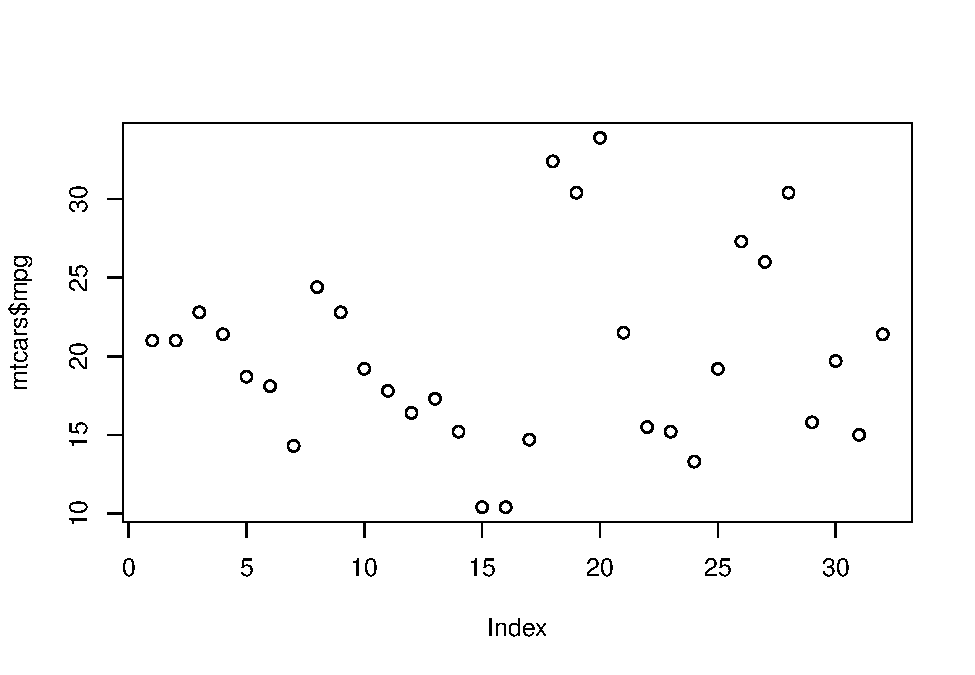
\includegraphics{Untitled_files/figure-latex/fig2-1.pdf}
\caption{Another sample figure}
\end{figure}

You can use \textbf{bookdown} to allow references for Tables and
Figures.

\hypertarget{tables}{%
\subsection{Tables}\label{tables}}

Below we can see how to use tables.

See awesome Table\textasciitilde{}\ref{tab:table} which is written
directly in LaTeX in source Rmd file.

\begin{table}
 \caption{Sample table title}
  \centering
  \begin{tabular}{lll}
    \toprule
    \multicolumn{2}{c}{Part}                   \\
    \cmidrule(r){1-2}
    Name     & Description     & Size ($\mu$m) \\
    \midrule
    Dendrite & Input terminal  & $\sim$100     \\
    Axon     & Output terminal & $\sim$10      \\
    Soma     & Cell body       & up to $10^6$  \\
    \bottomrule
  \end{tabular}
  \label{tab:table}
\end{table}

You can also use R code for that.

\begin{Shaded}
\begin{Highlighting}[]
\NormalTok{knitr}\SpecialCharTok{::}\FunctionTok{kable}\NormalTok{(}\FunctionTok{head}\NormalTok{(mtcars), }\AttributeTok{caption =} \StringTok{"Head of mtcars table"}\NormalTok{)}
\end{Highlighting}
\end{Shaded}

\begin{longtable}[]{@{}
  >{\raggedright\arraybackslash}p{(\columnwidth - 22\tabcolsep) * \real{0.2609}}
  >{\raggedleft\arraybackslash}p{(\columnwidth - 22\tabcolsep) * \real{0.0725}}
  >{\raggedleft\arraybackslash}p{(\columnwidth - 22\tabcolsep) * \real{0.0580}}
  >{\raggedleft\arraybackslash}p{(\columnwidth - 22\tabcolsep) * \real{0.0725}}
  >{\raggedleft\arraybackslash}p{(\columnwidth - 22\tabcolsep) * \real{0.0580}}
  >{\raggedleft\arraybackslash}p{(\columnwidth - 22\tabcolsep) * \real{0.0725}}
  >{\raggedleft\arraybackslash}p{(\columnwidth - 22\tabcolsep) * \real{0.0870}}
  >{\raggedleft\arraybackslash}p{(\columnwidth - 22\tabcolsep) * \real{0.0870}}
  >{\raggedleft\arraybackslash}p{(\columnwidth - 22\tabcolsep) * \real{0.0435}}
  >{\raggedleft\arraybackslash}p{(\columnwidth - 22\tabcolsep) * \real{0.0435}}
  >{\raggedleft\arraybackslash}p{(\columnwidth - 22\tabcolsep) * \real{0.0725}}
  >{\raggedleft\arraybackslash}p{(\columnwidth - 22\tabcolsep) * \real{0.0725}}@{}}
\caption{Head of mtcars table}\tabularnewline
\toprule
\begin{minipage}[b]{\linewidth}\raggedright
\end{minipage} & \begin{minipage}[b]{\linewidth}\raggedleft
mpg
\end{minipage} & \begin{minipage}[b]{\linewidth}\raggedleft
cyl
\end{minipage} & \begin{minipage}[b]{\linewidth}\raggedleft
disp
\end{minipage} & \begin{minipage}[b]{\linewidth}\raggedleft
hp
\end{minipage} & \begin{minipage}[b]{\linewidth}\raggedleft
drat
\end{minipage} & \begin{minipage}[b]{\linewidth}\raggedleft
wt
\end{minipage} & \begin{minipage}[b]{\linewidth}\raggedleft
qsec
\end{minipage} & \begin{minipage}[b]{\linewidth}\raggedleft
vs
\end{minipage} & \begin{minipage}[b]{\linewidth}\raggedleft
am
\end{minipage} & \begin{minipage}[b]{\linewidth}\raggedleft
gear
\end{minipage} & \begin{minipage}[b]{\linewidth}\raggedleft
carb
\end{minipage} \\
\midrule
\endfirsthead
\toprule
\begin{minipage}[b]{\linewidth}\raggedright
\end{minipage} & \begin{minipage}[b]{\linewidth}\raggedleft
mpg
\end{minipage} & \begin{minipage}[b]{\linewidth}\raggedleft
cyl
\end{minipage} & \begin{minipage}[b]{\linewidth}\raggedleft
disp
\end{minipage} & \begin{minipage}[b]{\linewidth}\raggedleft
hp
\end{minipage} & \begin{minipage}[b]{\linewidth}\raggedleft
drat
\end{minipage} & \begin{minipage}[b]{\linewidth}\raggedleft
wt
\end{minipage} & \begin{minipage}[b]{\linewidth}\raggedleft
qsec
\end{minipage} & \begin{minipage}[b]{\linewidth}\raggedleft
vs
\end{minipage} & \begin{minipage}[b]{\linewidth}\raggedleft
am
\end{minipage} & \begin{minipage}[b]{\linewidth}\raggedleft
gear
\end{minipage} & \begin{minipage}[b]{\linewidth}\raggedleft
carb
\end{minipage} \\
\midrule
\endhead
Mazda RX4 & 21.0 & 6 & 160 & 110 & 3.90 & 2.620 & 16.46 & 0 & 1 & 4 &
4 \\
Mazda RX4 Wag & 21.0 & 6 & 160 & 110 & 3.90 & 2.875 & 17.02 & 0 & 1 & 4
& 4 \\
Datsun 710 & 22.8 & 4 & 108 & 93 & 3.85 & 2.320 & 18.61 & 1 & 1 & 4 &
1 \\
Hornet 4 Drive & 21.4 & 6 & 258 & 110 & 3.08 & 3.215 & 19.44 & 1 & 0 & 3
& 1 \\
Hornet Sportabout & 18.7 & 8 & 360 & 175 & 3.15 & 3.440 & 17.02 & 0 & 0
& 3 & 2 \\
Valiant & 18.1 & 6 & 225 & 105 & 2.76 & 3.460 & 20.22 & 1 & 0 & 3 & 1 \\
\bottomrule
\end{longtable}

\hypertarget{lists}{%
\subsection{Lists}\label{lists}}

\begin{itemize}
\tightlist
\item
  Item 1
\item
  Item 2
\item
  Item 3
\end{itemize}

\hypertarget{refs}{}
\begin{CSLReferences}{1}{0}
\leavevmode\vadjust pre{\hypertarget{ref-hadash2018estimate}{}}%
Hadash, Guy, Einat Kermany, Boaz Carmeli, Ofer Lavi, George Kour, and
Alon Jacovi. 2018. {``Estimate and Replace: A Novel Approach to
Integrating Deep Neural Networks with Existing Applications.''}
\emph{arXiv Preprint arXiv:1804.09028}.

\leavevmode\vadjust pre{\hypertarget{ref-kour2014fast}{}}%
Kour, George, and Raid Saabne. 2014a. {``Fast Classification of
Handwritten on-Line Arabic Characters.''} In \emph{Soft Computing and
Pattern Recognition (SoCPaR), 2014 6th International Conference of},
312--18. IEEE.

\leavevmode\vadjust pre{\hypertarget{ref-kour2014real}{}}%
---------. 2014b. {``Real-Time Segmentation of on-Line Handwritten
Arabic Script.''} In \emph{Frontiers in Handwriting Recognition (ICFHR),
2014 14th International Conference on}, 417--22. IEEE.

\end{CSLReferences}

\bibliographystyle{unsrt}
\bibliography{references.bib}


\end{document}
